\documentclass[11pt, a4paper, twoside]{amsart} %The "twoside" here is for the headers to work

\usepackage{amsmath}
\usepackage{amsthm}
\usepackage{amssymb}
\usepackage{amsfonts}
\usepackage{graphicx}
\usepackage{latexsym}
%\usepackage{marvosym}
\usepackage{hyperref}
\usepackage{tikz-cd}
\usepackage{float}
\usepackage{color}
\usepackage[hmargin=1.9cm, vmargin=2cm, headsep=0.4cm]{geometry}
%\usepackage{titlesec} %This is for formatting the section headers

%\titleformat{\section}  %This is responsible for the change in the format of the section headings
%{\center\normalfont\Large\bfseries}
%{\thesection .\hskip 9pt}
%{0pt}
%{}

\renewcommand*{\thepage}{\scriptsize\arabic{page}} %This changes the font size of the page number in the first page

\usepackage{fancyhdr} %This is for the headers

\pagestyle{fancy}

\fancyhf{}
\fancyhead[CE]{\scriptsize {MICHAIL SAVVAS}} %Center header - pages with even number
\fancyhead[CO]{\scriptsize {AI AGENT FOR BACKGAMMON}} %Center header - pages with odd number
\fancyhead[RE,LO]{} %Right-even header, Left-odd header
\fancyhead[LE,RO]{\scriptsize \thepage} %Left-even header, Right-odd header - this is the page number
\renewcommand{\headrulewidth}{0pt} %These two are the sizes of the lines separating the headers
\renewcommand{\footrulewidth}{0pt} %from the text. I have removed them.

\usepackage{mathtools}
\usepackage{natbib}
\usepackage{cite}
\usepackage{color}

\newcommand{\fX}{\mathfrak{X}}
\newcommand{\bL}{\mathbb{L}}
\newcommand{\R}{\mathbb{R}}
\newcommand{\C}{\mathbb{C}}
\newcommand{\A}{A^{\bullet}}
\newcommand{\B}{B^{\bullet}}
\newcommand{\poly}{\mathbb{C}[t]}
\newcommand{\fM}{\mathfrak{M}}
\newcommand{\dspec}{{\textbf{Spec}}}
\newcommand{\rel}{\text{rel}}

\newtheorem{theorem}{Theorem}[section]
\newtheorem{lemma}[theorem]{Lemma}
\newtheorem{proposition}[theorem]{Proposition}
\newtheorem{corollary}[theorem]{Corollary}
\theoremstyle{definition}
\newtheorem{definition}[theorem]{Definition}
\newtheorem{note}[theorem]{Note}

\setlength{\parindent}{0pt}

\author{\footnotesize{MICHAIL SAVVAS}}
\date{}

\title{\textbf{CS 221 FALL 2015 PROJECT FINAL REPORT:\\ AI AGENT FOR BACKGAMMON}} 

\begin{document}

\maketitle

\begin{abstract}
\vspace*{-1cm} The goal of this project is to develop a smart AI agent to play backgammon. We follow Gerald Tesauro's approach and use reinforcement learning with a sigmoid linear evaluation function and a neural network evaluation function.\\
\end{abstract}

By turning in this assignment, I agree by the Stanford honour code and declare
that all of this is my own work.

\section{Introduction: Setup and Conventions}

\text{} \newline
\begin{minipage}{0.4\textwidth}
\begin{figure}[H]
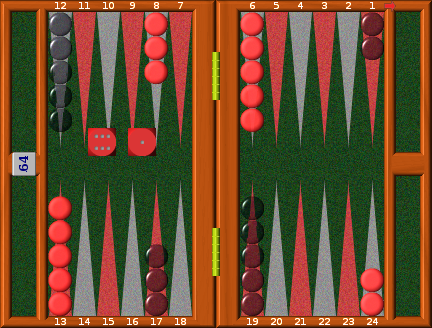
\includegraphics[width=0.9\textwidth]{StartingPosition}
Starting Position: The red checkers move clockwise and the black ones counteclockwise.
\end{figure}
\end{minipage}  
\begin{minipage}{0.6\textwidth}
Backgammon is one of the oldest board games for two players. The playing pieces (or checkers) are moved according to the roll of two dice, and a player wins by removing all of their checkers from the board before their opponent.\\
Detailed rules, terminology and notation for the game can for example be found here: \citep{WikiBG}, \citep{WikiN}.\\
For simplicity, convenience and also computational feasibility, we will consider games of backgammon \textbf{without a doubling cube} and \textbf{ignore the possibility of a gammon or backgammon}. The latter is a rare occurence in practice.\\
As can be seen in the figure, we denote the possible positions (points) by numbers $1$-$24$ and moves by pairs of numbers separated by a slash. For example, the move 12/18 17/18 creates an anchor (or block) at point 18 for black. A * next to a number indicates that one of the opponent pieces is hit through that move.
\end{minipage}



\section{Aim and Scope of Project}

The \textbf{aim} of the project is to design an AI agent that plays backgammon at the highest possible level of competence given the temporal and computational limitations of the project.\\
In particular, the agent should be able to take as \textbf{input} a board position and a dice roll and \textbf{output} the best possible move that the player can make.\\
We will use three \textbf{evaluation metrics} for our agent (see below):
\begin{enumerate}
\item \textbf{Performance} against the \textbf{baseline}.
\item \textbf{Ranking} of possible \textbf{moves}, compared to that of the \textbf{oracle}.
\item \textbf{Speed}.
\end{enumerate}
We will examine more closely the second metric. We are interested in performing an analysis of the game and its strategies based on our agent, the oracle and the comparison of the two, as well as personal experience. Of course, the first metric will be relevant to this analysis, as the better our agent performs against the baseline the bigger the overlap we expect to see with the oracle.\\
Speed is also important as a major technical obstacle we need to deal with and will limit our ability to search deep enough in the game tree.

\section{Modeling the game, Baseline and Oracle}

Our way of formalizing a game of backgammon will be to treat it as a Markov decision process (MDP), which essentially amounts to a search problem if we ignore the randomness provided to the game by the rolls of the dice.\\
Our MDP is the following:\\
\begin{itemize}
\item \textbf{Players:} \emph{Black} and \emph{red}.
\item \textbf{States $s$:} Triples $s$ = (\emph{board}, \emph{roll}, \emph{player}) where \emph{board} denotes the current configuration of the pieces, \emph{roll} the current dice roll and \emph{player} the player whose turn it is.
\item \textbf{Actions($s$) and Succ($s$, $a$):} If $s$ = (\emph{board}, \emph{roll}, \emph{player}) with \emph{player} = \emph{black} or \emph{red}, then the actions $a$ are the legal moves for the corresponding player given the situation of the \emph{board} and the \emph{roll} of the dice. The successor states in this case are Succ($s$, $a$) = $\lbrace$ (\emph{newBoard}, \emph{newRoll}, \emph{newPlayer}) $\rbrace$ where \emph{newBoard} denotes the new configuration of the pieces, \emph{newRoll} any possible roll and \emph{newPlayer} is now the other player.
\item \textbf{Transition probabilities T($s$, $a$, $s'$):} We have for every $s' \in$ Succ($s$, $a$) that T($s$, $a$, $s'$) $= \frac{1}{21}$ since all $21$ possible rolls occur with equal probability (we are assuming the dice are fair after all).
\item \textbf{Terminal states:} IsEnd($s$) = $1$ if and only if the \emph{board} only contains pieces of one colour.
\item \textbf{Rewards:} Since backgammon is a game, only terminal states will yield a reward and our convention will be that a black win gives reward $3$ and a red win reward $-3$. In other words, for $s$ = (\emph{board}, \emph{roll}, \emph{player}) we have Reward($s$) = $3$ if IsEnd($s$), \emph{board} contains no black pieces and \emph{player} = \emph{red} and similarly for the other case.\\
\end{itemize}

Our \textbf{baseline} algorithm will be the \textbf{random} policy:\\
\texttt{Pick an action $a \in $ Actions($s$) randomly with uniform probability.\\}
Our \textbf{oracle} will be the AI agent \textbf{GNU Backgammon} \citep{GnuBG}, which is one of the best AI agents for backgammon availabe and can achieve world class performance and game analysis.

\section{Approach towards building a competent AI agent : TD - Learning}

Our approach towards building a competent AI agent is largely based on Gerald Tesauro' s method of developing TD-Gammon in \citep{TDGammon} and \citep{TDGammon2}. The strategy proceeds as follows:
\begin{itemize}
\item Choose an appropriate feature vector $\phi(s)$ to assign to each state $s$ and an evaluation function $\text{Eval}(s, w)$ for each state $s$ given weights $w$ for the features $\phi$.
\item Initialize the weights (either set them to zero or uniformly randomly in the interval $[-1, 1]$). Then run simulations of the game, where the black player always takes the action that maximizes the expected value of the evaluation function of the successor state and the red player the one that minimizes the same expected value. At each ply $(s, a, r, s')$ update the weights according to the TD-Learning rule:
$$ w \leftarrow w - \eta \left( \text{Eval}(s, w) - \text{Reward}(s') - \text{Eval}(s', w) \right) \nabla_{w} \text{Eval}(s, w)$$ 
Note that we are using a discount factor $\gamma = 1$ throughout the project.
\item After completing the simulations and training the weights through self-play, our agent will perform a minimax search (or rather expectiminimax) in the game tree to a given depth to determine which is the best move. To be more concrete, we use the standard minimax recursion:
\[ \text{minimax}(s, d) = \begin{cases}
		\max_{a \in \text{Actions}(s)} \sum_{s' \in \text{Succ}(s,a)} \frac{1}{21} \text{minimax}(s', d - 1) \ \text{if} \ \text{\emph{player}}(s) = \text{\emph{black}} \\
		\min_{a \in \text{Actions}(s)} \sum_{s' \in \text{Succ}(s,a)} \frac{1}{21} \text{minimax}(s', d - 1) \ \text{if} \ \text{\emph{player}}(s) = \text{\emph{red}} \\
		\text{Eval}(s, w)  \ \text{if} \ d=0 \\
		\text{Reward}(s)  \ \text{if} \ \text{IsEnd}(s)
		\end{cases}
		\]
\end{itemize}
The biggest gain from TD-Learning is that by using sufficiently generic features and not employing any existing database of backgammon games or hard-coding some universally acceptable moves or domain specific knowledge into the agent, the end result is largely free of any human bias and thus more likely to detect new strategies or play in novel ways. Of course, having no need for external data is another plus.\\
We use the same features as Tesauro: For a state $s$ we have $192 + 2 + 2 + 2 = 198$ features.\\
The first $192$ correspond to counting pieces at every point. In particular, for every point $p$ and number $1 \leq n \leq 3$ we have one indicator feature for each player, which is equal to $1$ if the player has at least $n$ pieces at point $p$. For $n = 4$, we have the same feature, but its value equals $\frac{m-3}{2}$ where $m$ is the number of pieces that the player has at point $p$.\\
Then we have a feature for the bar for each player, whose value equals $\frac{m}{2}$ where $m$ is the number of pieces on the bar that belong to the player.\\
There are two more features that record the pieces whose have been borne off and their values are the percentages of the pieces of each player that are out of the game.\\
Finally, there are two indicator features recording which player's turn it is.\\
Let us denote the standard sigmoid function by $\sigma(x) = \frac{1}{1 + e^{-x}}$.\\ In this project, we make use of these features to cook up an evaluation function in the following two ways:
\begin{itemize}
\item \textbf{(Sigmoid linear)} This is a very simple evaluation function, given by $$\text{Eval}(s, w) = \sigma \left( w \cdot \phi(s) \right)$$
\item \textbf{(Neural network)} This is the neural network used by Gerald Tesauro. We use the $198$ weights as layer 0 input nodes. These are fully connected to $50$ hidden layer 1 intermediate nodes, each of which also has a bias feature. Then these $50$ nodes are connected to the final layer 2 output node, which has a bias feature of its own as well. At each step, we apply the sigmoid function, as is customary. The network is shown in the following figure.
\end{itemize}
\begin{figure}[H]
  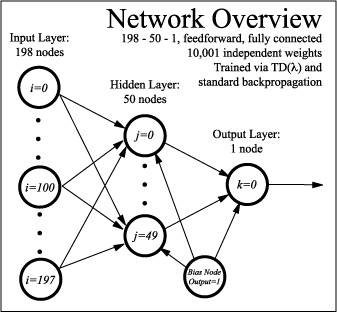
\includegraphics[width=0.4\linewidth]{NeuralNet.jpg}
  %\caption{Tesauro's neural network}
  \label{fig:boat1}
\end{figure}
We know that the neural network will give us a sensible agent after careful implementation and sufficient training, that was after all Tesauro's breakthrough. However, we examine the first case as well in order to see how far essentially a linear classifier can go as to capturing the mechanics of the game of backgammon.

\section{Results I : Performance against the Baseline}

For the \textbf{sigmoid linear} evaluation function, we obtain the following sets of weights through self-play and reinforcement learning:
\begin{itemize}
\item \textbf{(Set I)} We simulate 16.424 games. We initialize the weights uniformly randomly in the interval $[-1, 1]$. We normalize the weights every $100$ games and have a final reward of $3$ throughout. For the first 10.000 we use a constant $\eta = 0.1$ and for the last 6.424, we set $\eta = \frac{1}{1 + [i/250]}$ where $i$ is the count of the iterations (starting from $1$).
\item \textbf{(Set II)} We simulate 40.000 games. We initialize the weights uniformly randomly in the interval $[-1, 1]$. We normalize the weights every $100$ games throughout. For the first 10.000 games the reward is $3$, the next 15.000 $30$ and the last 15.000 $50$ (the reward does not really affect the result, but we opted for a change to see if anything new would happen). For the first 10.000 games we use a constant $\eta = 0.1$ and for the last 30.000 we set $\eta = \frac{1}{1 + [i/500]}$ where the counter $i$ is set to $0$ after 15.000 games.
\end{itemize}
We then use our \textbf{minimax} agent with search depth $1$ or $2$ to play against an opponent following the baseline random policy. The results are as follows:
\begin{center}
\begin{tabular}{ | c | c | c | c | c | }
\hline
\texttt{set} & \texttt{no of plies} & \texttt{no of games} & \texttt{percentage of minimax wins vs random} & \texttt{minimax player}\\ \hline
I & 1 & 2500 & 0.498000 & \texttt{black}\\ \hline
I & 1 & 3001 & 0.599000 & \texttt{random}\\ \hline
I & 1 & 3000 & 0.676333 & \texttt{red}\\ \hline
I & 2 & 500 & 0.502000 & \texttt{black}\\ \hline
I & 2 & 115 & 0.573913 & \texttt{red}\\ \hline
II & 1 & 10000 & 0.511600 & \texttt{black}\\ \hline
II & 1 & 10000 & 0.660400 & \texttt{red}\\ \hline
II & 2 & 300 & 0.550000 & \texttt{black}\\ \hline
\end{tabular}
\end{center}
%\textbf{Percentage of minimax wins vs random, Set I, 1-ply, 500 games: 0.555556}\\
%\textbf{Percentage of minimax wins vs random, Set I, 1-ply, 2000 games: 0.483500}\\
%\textbf{Percentage of minimax wins vs random, Set I, 2-ply, 500 games: 0.502000}\\
%\textbf{Percentage of minimax wins vs random, Set II, 1-ply, 10000 games: 0.511600}\\
%\textbf{Percentage of minimax wins vs random, Set II, 2-ply, 300 games: 0.550000}\\
%MAYBE DO MORE SET II 2-ply? DO NEURAL AFTER\\
\text{}\\
For the \textbf{neural network} evaluation function, we obtain the following sets of weights:
\begin{itemize} 
\item \textbf{(Set I)} We simulate 9.152 games. We initialize the weights to $0$. This forces a lot of weights to be equal to each other, identifying essentially all the layer 1 nodes. The reward is $3$, we don't normalize the weights and we set $\eta = \frac{1}{1 + [i/2000]}$, where $i$ counts the games simulated.
\item \textbf{(Sets I.5, II)} We simulate 7002 games. We initialize the weights uniformly randomly in the interval $[-1, 1]$. The reward is $3$, we don't normalize and set $\eta = \frac{1}{1 + [i/2000]}$, where $i$ counts the games simulated. In this way we obtain Set II of weights. We also record the weights after 5.109 games and these give us Set I.5.
\end{itemize}
Then analogously to the above we get the table:
\begin{center}
\begin{tabular}{ | c | c | c | c | c | }
\hline
\texttt{set} & \texttt{no of plies} & \texttt{no of games} & \texttt{percentage of minimax wins vs random} & \texttt{minimax player}\\ \hline
I & 1 & 2000 & 0.528500 & \texttt{random}\\ \hline
I.5 & 1 & 2034 & 0.551622 & \texttt{random}\\ \hline
II & 1 & 2006 & 0.546361 & \texttt{random}\\ \hline
\end{tabular}
\end{center}

\section{Results II : Comparison to Oracle}

For economy of space, we use the starting position and a few rolls as our reference. For the \textbf{sigmoid linear} evaluation function we have the following results for the \textbf{black} player:
\begin{center}
\begin{tabular}{ | c | c | c | c | c | c | }
\hline
\texttt{roll} & \texttt{GNU} & \texttt{set I, 1-ply} & \texttt{set I, 2-ply} & \texttt{set II, 1-ply} & \texttt{set II, 2-ply}\\ \hline
5-4 & 1/5 12/17 & 12/17 17/21 & 12/17 17/21 & 12/17 17/21 & 12/17 17/21\\ \hline
6-1 & 12/18 17/18 & 17/18 17/23 & 17/18 17/23 & 17/18 17/23 & 17/18 17/23\\ \hline
5-2 & 1/3 12/17 & 12/17 17/19 & 12/14 12/17 & 1/3 17/22 & 1/3 17/22\\ \hline
6-3 & 1/7 12/15 & 17/20 17/23 & 12/18 18/21 & 17/20 17/23 & 17/20 17/23\\ \hline
6-4 & 1/7 12/16 & 17/21 17/23 & 17/21 17/23 & 17/21 17/23 & 17/21 17/23\\ \hline
3-1 & 17/20 19/20 & 17/18 17/20 & 12/15 15/16 & 17/18 17/20 & 17/18 17/20\\ \hline
2-1 & 1/2 12/14 & 17/18 17/19 & 1/2 2/4 & 17/18 17/19 & 17/18 17/19\\ \hline
\end{tabular}
\end{center}
\text{}\\
If we perform the same for the \textbf{red} player, we obtain:
\begin{center}
\begin{tabular}{ | c | c | c | c | c | c | }
\hline
\texttt{roll} & \texttt{GNU} & \texttt{set I, 1-ply} & \texttt{set I, 2-ply} & \texttt{set II, 1-ply} & \texttt{set II, 2-ply}\\ \hline
5-4 & 24/20 13/8 & 24/20 20/15 & 13/8 6/2 & 13/9 13/8 & 13/8 6/2\\ \hline
6-1 & 13/7 8/7 & 13/7 8/7 & 13/7 7/6 & 13/7 7/6 & 13/7 7/6\\ \hline
5-2 & 24/22 13/8 & 13/11 11/6 & 13/8 6/4 & 13/8 6/4 & 13/8 6/4\\ \hline
6-3 & 24/18 13/10 & 13/10 8/2 & 13/10 10/4 & 13/10 10/4 & 13/10 10/4\\ \hline
6-4 & 24/18 13/9 & 24/20 8/2 & 13/7 7/3 & 13/7 7/3 & 13/7 7/3\\ \hline
3-1 & 8/5 6/5 & 13/10 8/7 & 6/5 6/3 & 6/5 6/3 & 6/5 6/3\\ \hline
2-1 & 24/23 13/11 & 24/23 8/6 & 6/5 6/4 & 6/5 6/4 & 6/5 6/4\\ \hline
\end{tabular}
\end{center}
\text{}\\
For the \textbf{neural} evaluation function we have the following table for the \textbf{black} player:
\begin{center}
\begin{tabular}{ | c | c | c | c | c | c | }
\hline
\texttt{roll} & \texttt{GNU} & \texttt{set I, 1-ply} & \texttt{set I, 2-ply} & \texttt{set II, 1-ply} & \texttt{set II, 2-ply}\\ \hline
5-4 & 1/5 12/17 & 17/21 17/22 & 17/21 17/22 & 17/21 17/22 & 17/21 17/22\\ \hline
6-1 & 12/18 17/18 & 17/18 17/23 & 17/18 17/23 & 17/18 17/23 & 17/18 17/23\\ \hline
5-2 & 1/3 12/17 & 17/19 17/22 & 17/19 17/22 & 17/19 17/22 & 17/19 17/22\\ \hline
6-3 & 1/7 12/15 & 17/20 17/23 & 17/20 17/23 & 17/20 17/23 & 17/20 17/23\\ \hline
6-4 & 1/7 12/16 & 17/21 17/23 & 17/21 17/23 & 17/21 17/23 & 17/21 17/23\\ \hline
3-1 & 17/20 19/20 & 17/18 17/20 & 17/18 17/20 & 17/18 17/20 & 17/18 17/20\\ \hline
2-1 & 1/2 12/14 & 17/18 17/19 & 17/18 17/19 & 17/18 17/19 & 17/18 17/19\\ \hline
\end{tabular}
\end{center}
\text{}\\
For the \textbf{neural} evaluation function for \textbf{red} player we get:
\begin{center}
\begin{tabular}{ | c | c | c | c | c | c | }
\hline
\texttt{roll} & \texttt{GNU} & \texttt{set I, 1-ply} & \texttt{set I, 2-ply} & \texttt{set II, 1-ply} & \texttt{set II, 2-ply}\\ \hline
5-4 & 24/20 13/8 & 13/8 6/2 & 13/8 6/2 & 13/8 6/2 & 13/8 6/2\\ \hline
6-1 & 13/7 8/7 & 13/7 7/6 & 13/7 7/6 & 13/7 7/6 & 13/7 7/6\\ \hline
5-2 & 24/22 13/8 & 13/8 6/4 & 13/8 6/4 & 13/8 6/4 & 13/8 6/4\\ \hline
6-3 & 24/18 13/10 & 13/10 10/4 & 13/10 10/4 & 13/10 10/4 & 13/10 10/4\\ \hline
6-4 & 24/18 13/9 & 13/7 7/3 & 13/7 7/3 & 13/7 7/3 & 13/7 7/3\\ \hline
3-1 & 8/5 6/5 & 6/5 6/3 & 6/5 6/3 & 6/5 6/3 & 6/5 6/3\\ \hline
2-1 & 24/23 13/11 & 6/5 6/4 & 6/5 6/4 & 6/5 6/4 & 6/5 6/4\\ \hline
\end{tabular}
\end{center}

\section{Results III : Speed}

In this short section, we make a few comments about speed.\\
It turns out that due to the implementation of the game engine and the rest of the algorithms not trying to be as economical as possible and also possibly due to the number of features and the programming language being used (Python) and other not yet detected faults of the author, training the weights for the neural network required huge amounts of time. We obtained Set II of weights by running TD-Learning for more than 25 hours.\\
For similar reasons, running minimax for 2 plies also takes significant amounts of time, while depth 3 is very, very slow. For the neural network, even 1 ply requires moderate amounts of time.\\
We observe that the minimax computation for the red pieces is noticeably slower than the minimax computation for the black pieces.\\
These explain the numbers of simulations and the small number of games played against a random policy opponent in the above.

\section{Analysis and Comments}

We can proceed to quite a few observations from our results and experience from actually playing against the agent.\\
\\
\textbf{Observations based on perfomance against the baseline: } The first thing we can note is that with all sets of weights, the agent seems to perform significantly better when it plays the red pieces. We can probably attribute this to the effect of the initial simulations that require a great number of games to even out. We can see from the sigmoid linear case that there is a small trend for black wins to increase percentagewise and for red wins to decrease. We believe that with more simulations these two percentages will converge to the percentage we obtain when the minimax player is chosen randomly and which should be the average of the two, as it is roughly in the computed example too.\\
Another thing we can say is that there is a noticeable improvement compared to the random policy agent in most cases, where our minimax agent wins on average roughly 60\% of the time in the sigmoid linear case (1-ply) and 56\% for the neural network with Set I.5 or Set II and 53\% for Set I (1-ply). The latter difference is reasonable, since Set I was initialized with symmetric weights (all equal to 0) and therefore is expected to perform worse than Sets I.5 and II (which were initialized randomly) even though the simulations were more. It is however expected to outperform the sigmoid linear performance given more training, a tendency which is justified by its win percentage.\\
We do not have enough data to sufficiently compare the performance of 2-ply against 1-ply minimax, however there are indications that this gives a further improvement, as suggested by the perfomance of black for Set II in the sigmoid linear table.\\
Comparing the performance of the two evaluation functions to each other, we can say that even though the neural network weights were trained for less than 10.000 games (in the case of I.5 and II even more so) the performance of the neural network is only ever so slightly worse than the sigmoid linear, especially for the sets I.5 and II which were initialized more sensibly. With more learning, we are confident that the performance would be much better.\\
\\
\textbf{Observations based on comparison to oracle and gameplay: } We see that for all sets of weights there is, with very few exceptions, either partial or no overlap between the proposals of GNU and our minimax agent. This is because the number of simulated games is small and the agent has not yet captured key mechanics of backgammon.\\
Judging by the proposed moves, the agent seems to give priority to pieces in or close to its own homezone and does not try at all to protect its own pieces or form new blocks (again with few exceptions).\\ 
By actually playing against the agent ourselves, we can testify that this is indeed the case in general. The general strategy it follows, for all sets of weights provided, is to first move as many pieces inside as possible without really caring about its pieces being hit. However, it appears somewhat smarter during mid and late game. The agent is then more careful about how to move its pieces to the homezone and often it forms new blocks. Here the neural network seems to already perform better, as it makes smarter positional choices for the blocks it forms. Finally, during late game the agent is quite aggressive and usually hits the opponent given the chance.\\
We can describe the strategy developed by the agent as a ``wait and see" strategy: Try to move as many pieces to the homezone and into a good formation, don't worry about pieces being hit, wait at the opponent homezone and then hopefully hit the opponent back at the end and win.\\
We can probably say that the reason for the emergence of this strategy is that states that are close to being terminal have a greater effect on the agent's strategy during the initial simulations and our agent has not been trained enough to get rid of this initial ``bias".

\section{Challenges, Further Developments and Existing Agents}

By far the biggest challenge presented in backgammon is the large \textbf{branching factor} of the game tree, which makes searching through it  quickly nearly impossible. By way of comparison, the state space and branching factor for chess are approximately $10^{47}$ and 35, whereas for backgammon they are approximately $10^{20}$ and 250.\\
This is the primary reason for the speed issues we alluded to earlier, which did not allow us to perform more simulations and obtain better weights (given appropriate time constraints for this project).\\
Naturally, we could try to make our implementation as economical as possible, program it at a faster language than Python (e.g. C) and employ more computational power to obtain a more competent agent.\\
Other directions that might be worth pursuing are:
\begin{enumerate}
\item Providing options for the level of play of the agent, either by introducing some randomness or using the ranking of the possible moves according to their minimax values, and observing the differences in the strategy followed by the agent.
\item Applying temporal difference learning methods to build agents for other variants of backgammon. For example, such variants which are especially popular in Greece are ``plakoto" \citep{WikiPlakoto} and ``fevga".
\end{enumerate} 
%To tackle this challenge, we can use a combination of different techniques seen in class. It seems most fruitful to insert domain specific knowledge into the agent by way of introducing evaluation functions and then performing limited depth tree search together with alpha-beta pruning. In order to find a good evaluation function we have several options:\\
%We can perform function approximation and learn the weights either by existing datasets of backgammon games or by reinforcement learning. The weights can be chosen based on human experience and we can also use neural networks for the evaluation function to capture more complicated behaviours. We could also consider Monte Carlo approximation or reinforcement learning for the evaluation function directly to avoid any human bias whatsoever.\\
Various combinations of ideas and approaches have been carried out in the past with great success and impressive results. For economy of space, we just refer to the work of Hans Berliner \citep{Berliner} and Gerald Tesauro's Neurogammon \citep{NeuroG} and TD-Gammon \citep{TDGammon}, \citep{TDGammon2}. Our neural network approach, as already mentioned, closely follows the latter.\\
We also mention the world class program Palamedes, developed by Nikolaos Papahristou, \citep{Palamedes} which applies reinforcement learning techniques to various backgammon variants, including ``plakoto" and ``fevga". 

\bibliography{Master}
\bibliographystyle{alpha}

\end{document}